\chapter{Realisierung des Source-To-Source Compilers}
\label{chap:Realisierung}
Gestützt auf das grundsätzliche Wissen über Compiler, die herausgearbeiteten Unterscheidungen von  Xamarin.Forms und Flutter sowie die Differenzen der verwendeten Programmiersprachen  \Csharp und Dart, wird in diesem Kapitel die Realisierung des Source-To-Source Compilers. Um das Projekt mit Roslyn Integration zu implementieren,  bietet sich die \ac{ide} (deutsch Entwicklungsumgebung) Visual Studio 2019 an, da auf dieser Plattform Projekte angelegt werden können, die mit dem Roslyn Compiler interagieren. Die zu entwickelnde Projektmappe, anhand derer der Prototyp validiert werden soll, besteht also aus dem Source to Source Compiler mit Rosyln Integration, der grafischen Benutzeroberfläche und einer Xamarin.Forms Anwendung als Testobjekt wobei letzteres erst im nächsten Kapitel eingeführt wird. 



\section{Programmablauf}
Mit Hilfe des Roslyn Compilers kann der Source-To-Source Compiler Auswertungen zu den in der Xamarin.Forms App referenzierten Dateien durchführen.  Somit ist es möglich eine Auflistung aller verfügbaren Quelltextdokumente aus einem Projekt zu erhalten.  Diese Auswertung beinhaltet jedoch keine \ac{xaml}-Dateien,  da diese nicht von Roslyn behandelt werden.  Da jede \ac{xaml} Datei jedoch eine Codebehind-Datei mit der Dateiendung .XAML.CS beinhaltet können die  \ac{xaml} Dateien über das Dateisystem geladen werden.  Über diesen Wege kann sichergestellt werden, dass ausschließlich Dokumente übersetzt werden die Teil der Xamarin.Forms Anwendung sind, und nicht aus dem Projekt ausgeschlossen wurden und dennoch im Dateiverzeichnis verfügbar sind.  Nachdem der Source-To-Source Compiler alle gefunden Quelltextdateien übersetzt hat, und die Metadaten übernommen hat ist die Übersetzung  abgeschlossen.  Darauf basierend kann nun ein \ac{uml} Aktivitätsdiagramm angelegt werden,  welches den Übersetzungsvorgang visualisiert und in Abbildung \ref{fig:umlablauf} dargestellt ist.  

\begin{figure}[!ht]
 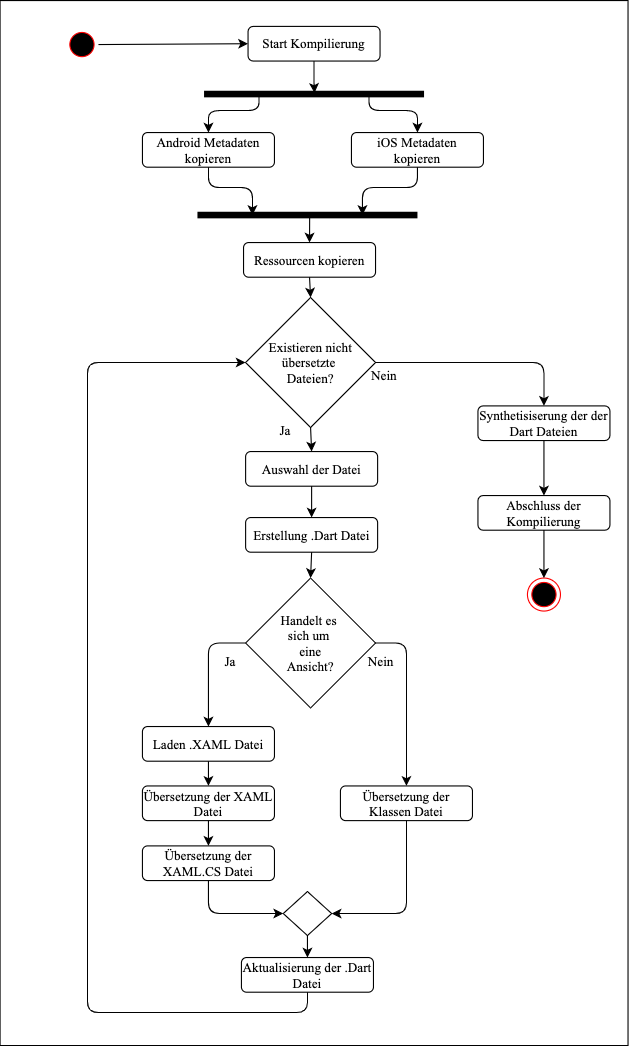
\includegraphics[width=\textwidth,keepaspectratio]{Images/Implementation/Ablauf.png}
 \caption{Aktivitätsdigramm}
 \label{fig:umlablauf}
\end{figure}
Das visualisierte \ac{uml}-Diagramm ist aufgrund der Komplexität des Compilers auf einer hohen Abstraktionsebene.  In den folgenden Abschnitten werden die einzelnen Aspekte der Kompilierung näher betrachtet. 


\section{Metadaten}
Wie das UML Diagramm visualisiert können die Metadaten von Android und iOS Metadaten parallel in die Flutter Anwendung kopiert werden können.  Da die Metadaten plattformspezifische Eigenschaften der mobilen Anwendungen sind,  wird im  folgenden die Details für beide Betriebssysteme eingegangen. 

\subsection{Android Metadaten}
Zu den Android spezifischen Metadaten gehören die sogenannten Launcher Icons,  die den Anwendern als App-Icon angezeigt werden.  Xamarin.Android speichert diese Bilder innerhalb des Android Projektes in Ordnern, welche die unterschiedlichen Pixeldichten der Android-Geräte unterstützen.  Da in diesen Ordnern unter Umständen viele Bilder liegen ist es notwendig das richtige Bild auszuwählen.  Innerhalb von Xamarin.Forms wird das Icon über die Klasse MainActivity.cs definiert wie dies in Quelltext  \ref{lst:IconName} dargestellt ist. 

\lstinputlisting[label={lst:IconName},caption={Xamarin.Forms Android Launcher-Icon Name}, language=csh]{SourceCode/IconName.cs}

Nach der Extraktion des Namens können nun die Bilder kopiert werden.  In dem von der Flutter SDK erzeugten App liegen bereits Bilder als Platzhalter für,  diese können einfach ausgetauscht werden. 

Der nächste wichtige Eigenschaft der Anwendung ist die sogenannte PackageID  dieser eindeutige Identifizierer  identifiziert die Anwendung auf dem Gerät sowie im Google-Play Store.  Es ist daher notwendig,  diese ID innerhalb der Flutter Anwendung wiederzuverwenden.  Die Information kann in Xamarin.Forms aus der AndroidManifest.XML Datei ausgelesen werden, jedoch ist es nicht ausreichend die Information in die Manifest Datei bei Flutter zu schreiben, da diese Information ebenfalls in andere Dateien wie die build.gradle hinterlegt werden muss. Es steht jedoch ein Plugin mit dem Namen change\_app\_package\_name zur Verfügung,  welches alle notwendigen Änderungen vornimmt.  Dafür muss das Plugin als Abhängigkeit zum Projekt hinzugefügt werden und kann anschließend über die Kommandozeile ausgeführt werden.

Einfacher ist die Übertragung des Anwendungsnamen,  der ebenfalls aus dem AppManifest extrahiert werden kann, im Gegensatz zur Package ID ist es jedoch ausreicht,  den Namen in die Flutter-Manifest Datei zu schreiben.  Im Gegensatz zu Xamarin.Forms gibt es bei Flutter jedoch 3 Manifest Dateien,  wobei ausschließlich die Datei im Verzeichnis 'Project/app/src/main' aktualisiert werden muss. 

Ein weiterer Inhalt des AppManifests sind die Berechtigungen,  welche die mobile Anwendung während der Laufzeit erfragen kann.  Diese können ebenfalls wie der Name kopiert werden. 

\subsection{iOS Metadaten}




\section{XAML zu Dart}



\section{C\# zu Dart}


Da sowohl die grafische Benutzeroberfläche als auch der Source-To-Source Compiler mit .Net Technologien realisiert wurden lassen sie sich einfach miteinander kombinieren.  Dafür erhält die  \ac{gui} eine Ahängigkeit auf das \ac{s2s}-Projekt.  



\section{Grafische Benutzeroberfläche}
Die \ac{gui} ist der zentrale Berührungspunkt von Anwendern mit dem Source-To-Source Compiler.  Er spielt soll die notwendigen Eingabe-Möglichkeiten anbieten,  das Ergebnis ausgeben und den Anwender auf mögliche Fehler hinweisen.  Als grafisches Vorbild soll auf das in Kapitel \ref{chap:CompilerEntwurf} entworfene Mockup zurückgegriffen werden.  Für die Erstellung einer grafischen Benutzeroberfläche stehen eine Vielzahl von Technologien mit verschiedenen Vor- und Nachteilen zur Verfügung.  Beispielsweise hätte eine Webseite den Vorteil,  das Anwender keinen Installationsaufwand haben und darüber hinaus auch Plattform-unabhängig auf den Compiler zugreifen können.  Jedoch bringen Webseiten neben dem eigentlichen Entwicklungsaufwand weitere Herausforderungen mit sich,  so haben potentielle Anwender nicht mehr die volle Kontrolle über ihren eigenen Quelltext, wenn sie diesen auf einer Webseite hochladen.  
Aus diesem Grunde,  wird die in dieser Arbeit entworfene Oberfläche eine lokale Anwendung sein,  die von Anwendern lokal installiert werden muss aber im Gegenzug garantiert,  dass niemand Zugriff auf den Source-Code von Anwendern erhält.  Zu diesem Zwecke wird die \ac{gui} mit der Technologie \ac{wpf} realisiert.  Dabei handelt es sich um ein \ac{ui}-Framework des .NET Frameworks welches für die Erstellung von Desktop Anwendungen geeignet ist und mit XAML und \Csharp entwickelt wird.  \footcite[Vgl.][S. 1f]{Wenger2012} Da die Build Tools für Visual Studio nur für Windows Computer ist es auch keine Einschränkung,  dass Anwendungen die mit \ac{wpf} realisiert werden ausschließlich unter diesem Betriebssystem ausführbar sind.

In der Zukunft könnte der Source to Source Compiler auch eine Web-Oberfläche bekommen,  diese hätte die zwei folgenden essentielle Vorteile im Gegensatz zu der aktuellen Implementierung.  Reduktion des Installationsaufwandes - durch den Betrieb über eine Webseite könnte die Installation von der Anzeige entkoppelt werden.  Natürlich wäre eine Client-Server Struktur auch ohne eine Webseite erreichbar,  jedoch haben Webseiten darüber hinaus den zusätzlichen Vorteil,  dass sie Plattform-unabhängig zur Verfügung stehen,  was es zum Beispiel für Xamarin.Forms Entwickelr mit einem Mac OSX Computer erlauben würde ebenfalls von dem Compiler zu profitieren, ohne sich eine Windows Installation vornehmen zu müssen
